\pagestyle{empty}
\centering
\fontsize{2cm}{2cm}\selectfont{System Requirements Document} \\
\vspace{2mm}
\fontsize{1cm}{1cm}\selectfont Audio digital signal processor \\
\vspace{2mm}
\large BeCreative Minor\\
\normalsize
\vspace{4cm}
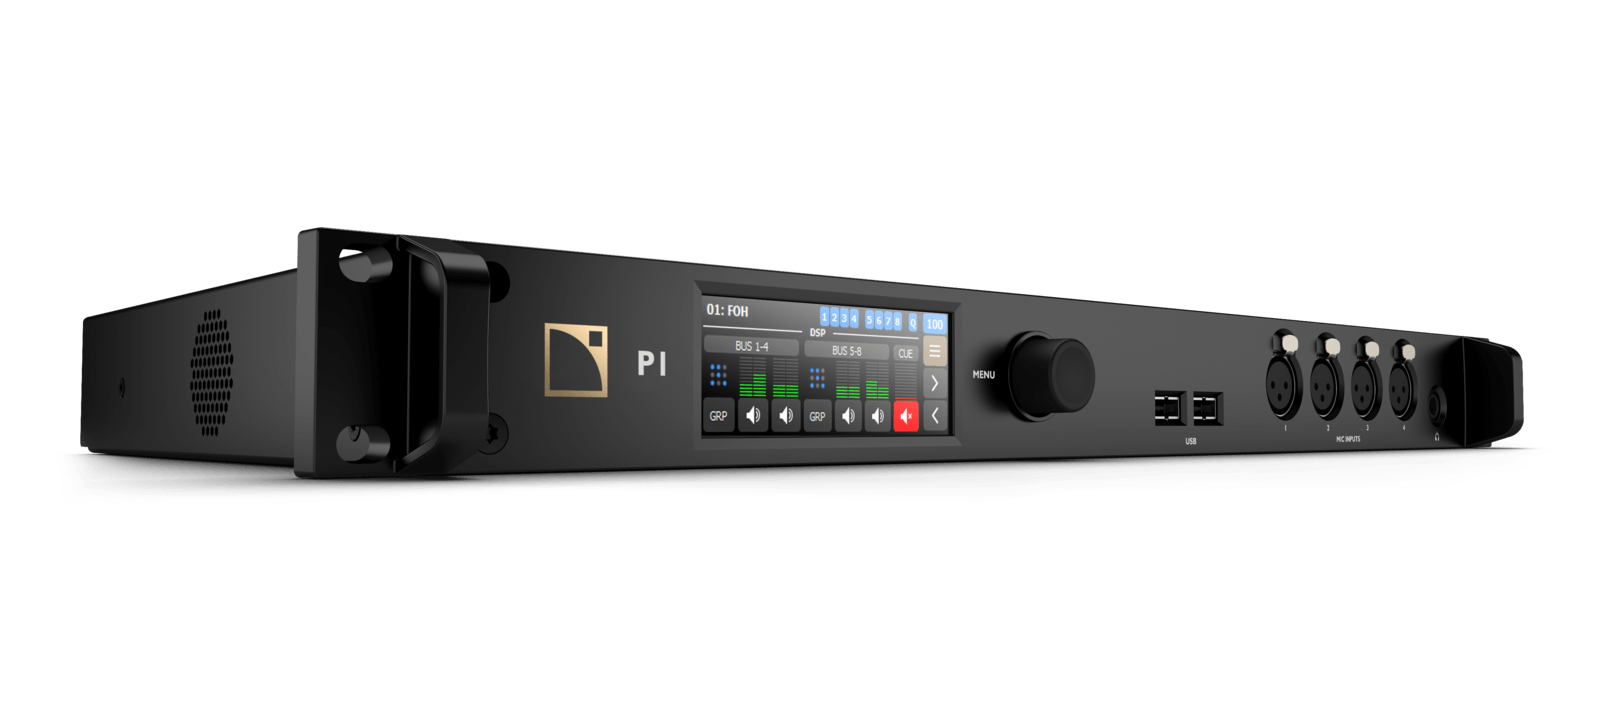
\includegraphics[width=\linewidth]{3DR_P1_Perspective.png}\\
\vfill
\normalsize Busse Lommers \\
Robin van den Dungen \\
Mahmud Gürler \\
Silas Kamphuis \\
Hein Verhallen \\
Youri Tils \\
Ahmed Abdelrahim \\
Fontys Hogescholen, De Rondom 1, 5612 AP Eindhoven \\
\today

\begin{justify}


\newpage
\tableofcontents
\thispagestyle{empty}

\newpage
\pagestyle{plain}
\setcounter{page}{1}

\chapter*{Abbreviation List}

\begin{table}[!h]
	\centering
\begin{tabular}{|c|c|}
	\hline
\textbf{Abbreviation} & \textbf{Explanation}        	\\ \hline
DAC                   & Digital to analog converter 	\\ \hline
ADC                   & Analog to digital converter 	\\ \hline
RAM                   & Random acces memory 			\\ \hline
SINAD                 & Signal to noise and distortion 	\\ \hline
TRS                   & Tip ring sleeve connector(Jack)	\\ \hline
FPGA                  & Field programmable gate array 	\\ \hline
\end{tabular}
\caption{List of commonly used Abbreviations}
\label{Abbreviation list}
\end{table}